\documentclass[3p,authoryear,fleqn]{elsarticle}
\journal{NeuroImage}

\usepackage[mode=buildnew]{standalone}
\usepackage{gincltex}
\usepackage{glossaries}
\usepackage{booktabs} \usepackage{multirow}
\usepackage[colorinlistoftodos]{todonotes}
\usepackage{xifthen}
\usepackage{xspace}
\usepackage{graphicx}
\graphicspath{{figures/}}

\usepackage{amsmath}
\usepackage{amssymb}
\DeclareMathOperator{\tr}{tr}
\DeclareMathOperator{\argmax}{argmax}
\DeclareMathOperator{\argmin}{argmin}
\DeclareMathOperator{\diag}{diag}
\DeclareMathOperator{\dist}{dist}
\DeclareMathOperator{\const}{Const.}
\providecommand{\e}[1]{\ensuremath{\times 10^{#1}}}
\providecommand{\mdist}[2]{ \mathcal{D}_{#2}^2(\mathbf{#1}) }
\providecommand{\omegaset}{\ensuremath{\boldsymbol{\Omega}}}
\providecommand{\gammaset}{\ensuremath{\boldsymbol{\Gamma}}}
\providecommand{\regseg}{\emph{regseg}}
\providecommand{\Regseg}{\emph{Regseg}}
\providecommand{\lowb}{\textit{b0}}

\let\oldhat\hat
\renewcommand{\vec}[1]{\mathbf{#1}}

\providecommand{\nvec}[1]{\hat{\mathbf{#1}}}
\providecommand{\suppl}[1]{\href{http://figshare.com/s/459c26b4ee8211e493b306ec4bbcf141}{Supplemental Materials}, #1}
\providecommand{\isores}[2][]{#2\ensuremath{\times}#2\ensuremath{\times}#2\ifthenelse{\equal{#1}{}}{}{ [#1]}\xspace}

\usepackage{url}
\usepackage[colorlinks=true,linkcolor=black, citecolor=blue, urlcolor=blue]{hyperref}
\usepackage{doi}

\hyphenation{op-tical net-works semi-conduc-tor an-isot-ropy regis-tra-tion iso-tropic Free-Surfer align-ed pre-sent work-flow data-set data-sets}

\makeatletter{}\newacronym{mr}{MR}{magnetic resonance}
\newacronym{mri}{MRI}{magnetic resonance imaging}
\newacronym{dwi}{DWI}{diffusion weighted image}
\newacronym{dmri}{dMRI}{diffusion MRI}
\newacronym{dw}{DW}{diffusion weighted}
\newacronym{dti}{DTI}{diffusion tensor image}
\newacronym{t1}{T1w}{T1 weighted}
\newacronym{t2}{T2w}{T2 weighted}
\newacronym{csf}{CSF}{cerebrospinal fluid}
\newacronym{wm}{WM}{white matter}
\newacronym{gm}{GM}{grey matter}
\newacronym{epi}{EPI}{echo-planar imaging}
\newacronym{gre}{GRE}{gradient echo sequence}
\newacronym{fa}{FA}{fractional anisotropy}
\newacronym{md}{MD}{mean diffusivity}
\newacronym{adc}{ADC}{apparent diffusion coefficient}
\newacronym{acwe}{ACWE}{active contours without edges}
\newacronym{adf}{ADF}{active deformation field}
\newacronym{map}{MAP}{maximum a posteriori}
\newacronym{snr}{SNR}{signal-to-noise ratio}
\newacronym{pve}{PVE}{partial volume effect}
\newacronym{roi}{ROI}{region of interest}
\newacronym{mrf}{MRF}{Markov Random Field}
\newacronym{pde}{PDE}{partial differential equation}
\newacronym{swindex}{sWI}{surface warping index}
\newacronym{wi}{WI}{Warping index}
\newacronym{nof}{NoF}{number of fibers}
\newacronym{t2b}{T2B}{T2w-registration based}
\newacronym{fft}{FFT}{fast fourier transform}
\newacronym{hcp}{HCP}{Human Connectome Project}
\newacronym{pe}{PE}{phase-encoding}
\newacronym{ci}{CI}{confidence interval}

\makeglossaries

 

\usepackage[T1]{fontenc}
\usepackage{charter}

\usepackage{array}
\newcolumntype{L}[1]{>{\raggedright\let\newline\\\arraybackslash\hspace{0pt}}m{#1}}

\usepackage{ifpdf}

\ifpdf
  \usepackage[switch]{lineno}
  \else
  \makeatletter
  \def\temp{dvips.def}
  \ifx\Gin@driver\temp
  \def\Ginclude@graphics#1{\def\temp{#1}---image \expandafter\strip@prefix\meaning\temp---}
  \fi
  \makeatother
\fi


\def\bibsection{\section*{References}}
\begin{document}
\begin{frontmatter}


\title{Active contours-driven registration method for the structure-informed segmentation of diffusion MR images\tnoteref{t1}}
\tnotetext[t1]{Supplemental materials to this work will be publicly available upon publication with doi:\href{http://figshare.com/s/459c26b4ee8211e493b306ec4bbcf141}{10.6084/m9.figshare.1397502}.
During the review process, the document is available with the private link.}

\author[bit,ciber]{Oscar~Esteban\corref{corrauthor}}
\cortext[corrauthor]{Corresponding author}
\ead{phd@oscaresteban.es}
\author[ucla]{Dominique~Zosso}
\author[lts5]{Alessandro~Daducci}
\author[chuv,lts5]{Meritxell~Bach-Cuadra}
\author[bit,ciber]{Mar\'ia-J.~Ledesma-Carbayo}
\author[lts5]{Jean-Philippe~Thiran}
\author[bit,ciber]{Andres~Santos}


\address[bit]{Biomedical Image Technologies (BIT), ETSI Telecomunicaci\'on, Universidad Polit\'ecnica de Madrid, Madrid, Spain}
\address[ciber]{Centro de Investigaci\'on Biom\'edica en Red en Bioingenier\'ia, Biomateriales y Nanomedicina (CIBER-BBN), Spain}
\address[ucla]{Department of Mathematics, University of California,
Los Angeles (UCLA), Los Angeles, CA, US}
\address[lts5]{Signal Processing Laboratory (LTS5), \'Ecole Polytechnique
F\'ed\'erale de Lausanne (EPFL), Lausanne, Switzerland}
\address[chuv]{Dept. of Radiology, CIBM, University
Hospital Center (CHUV) and University of Lausanne (UNIL), Lausanne, Switzerland}


\begin{abstract}
\makeatletter{}Current applications of whole-brain tractography to \acrlong*{dmri} data require highly precise
  delineations of anatomical structures, which are usually projected from \acrlong*{t1} images
  by registration.
In this study, we propose \regseg{}, which is a simultaneous segmentation and registration method
  that uses active contours without edges extracted from structural images.
The contours evolve through a free-form deformation field supported by the B-spline basis
  to optimally map the contours onto the data in the target space.
We tested the functionality of \regseg{} using four digital phantoms warped with known and
  randomly generated deformations, where subvoxel accuracy was achieved.
We then applied \regseg{} to a registration/segmentation task using 16 real diffusion MRI
  datasets from the \acrlong*{hcp}, which were warped by realistic and nonlinear distortions that are typically
  present in these data.
We computed the misregistration error of the contours estimated by \regseg{} with respect
  to their theoretical location using the ground truth, thereby obtaining a 95\% CI of 0.56--0.66 mm
  distance between corresponding mesh vertices, which was below the 1.25 mm isotropic resolution of the images.
We also compared the performance of our proposed method with a widely used registration tool, which showed
  that \regseg{} outperformed this method in our settings. 
\end{abstract}

\begin{keyword}
active~contours \sep cortical~parcellation \sep diffusion MRI \sep nonlinear~registration \sep segmentation \sep susceptibility~distortion.
\end{keyword}

\end{frontmatter}

\linenumbers
\makeatletter{}\section{Introduction}\label{sec:regseg-introduction}
\Gls*{dmri} enables the mapping of microstructure \citep{basser_microstructural_1996}
  and connectivity \citep{craddock_imaging_2013} of the human brain \emph{in-vivo}.
It is generally acquired using \gls*{epi} schemes, since they are very fast at
  scanning a large sequence of images called \glspl*{dwi}, each sensitized with
  a gradient to probe proton diffusion in a certain orientation.
Subsequent processing involves describing the local microstructure with one available
  model, which ranges from the early \gls*{dti} proposed by \cite{basser_microstructural_1996}
  to current models such as \citep{daducci_accelerated_2015}.
The microstructural map is then used to draw the preferential orientations of diffusion
  across regions using tractography \citep{mori_threedimensional_1999}.
Finally, the streamlines found are filtered with a cortical parcellation
  to build the graph representing the corresponding structural
  network \citep{hagmann_mapping_2008}.
Since the proposal of the earliest methodologies to solve the three problems,
  there is a need for precisely identifying the anatomy on the \gls*{dmri} space.
In fact, current trends in reconstruction \citep{jeurissen_multitissue_2014} and
  tractography \citep{smith_anatomicallyconstrained_2012} are increasingly using
  structural information to improve the microstructural mapping and fiber-tracking.

The structural information required by pioneer tractography studies was a simple
  \gls*{wm} mask to provide with a termination criteria for the streamlines.
The first attempts to segment the \gls*{wm} in \gls*{dti} involved thresholding the
  \gls*{fa}\footnote{the \gls*{fa} is a scalar parameter of diffusion derived from
  the \gls*{dti}.} map.
However, the mask and subsequent analyses are highly dependent on the threshold set
  \citep{taoka_fractional_2009}.
To overcome the unreliability of \gls*{fa} thresholding, and to broaden
  \gls*{wm} segmentation to brain tissue segmentation, a large number of
  methods have been proposed using \glspl*{dwi}, the \lowb{}, and \gls*{dti}-derived
  scalar maps such as \gls*{fa}, \gls*{adc} and others \citep{zhukov_level_2003,
  rousson_level_2004,jonasson_segmentation_2005,liu_brain_2007,hadjiprocopis_unbiased_2005,
  lu_segmentation_2008,han_experimental_2009}.
However, the precise segmentation of \gls*{dmri} is difficult for several limitations.
First, \gls{dmri} images have a resolution that is much lower than that of the imaged
  microstructural features.
Therefore, voxels located in structural discontinuities are affected by partial
  voluming of the signal sources.
Second, the extremely low \gls*{snr} and the high dimensionality of the \glspl*{dwi} prevent
  their direct use in segmentation.
Third, the low contrast between \gls*{gm} and \gls*{wm} in the \lowb{} volumes also makes
  them unsuitable for brain tissue segmentation.

An alternative route to segmentation in native \gls*{dmri} space is the mapping of the
  structural information extracted from anatomical MR images, such as \gls*{t1}, through
  an image registration process.
Generally, intra-subject registration of MR images of the brain involves only a linear
  mapping to compensate for head motion between scans.
However, \gls*{epi} images speed up the acquisition process at the cost of introducing geometrical
  distortion, as well as signal degradation and destruction \citep{jezzard_correction_1995}.
The so-called \emph{\gls*{epi} distortions} have a major impact on the anatomy extracted
  from \gls*{dmri}, particularly in certain fiber bundles \citep{irfanoglu_effects_2012}.
To overcome this problem, two broad families of solutions are available.
First, it is possible to use an existing ``\gls*{epi} distortion correction''
  method to compensate for the nonlinear part of the misalignment with the structural space,
  combined with a rigid registration method.
Second, to apply a nonlinear registration method with specific constraints derived from the
  theoretical properties of the \gls*{epi} distortion.
However, both solutions require extra acquisitions to be included within the \gls*{dmri} scanning
  protocol, such as fieldmaps \citep{jezzard_correction_1995}, \glspl*{dwi} with a different
  \gls*{pe} scheme \citep{cordes_geometric_2000,chiou_simple_2000}, or \gls*{t2} images
  \citep{kybic_unwarping_2000}.
In the following, we will refer to this latter approach as \gls*{t2b} correction.
\Gls*{epi} corrections have been an active field of research, with numerous refinements and
  combinations of the original methods \citep{holland_efficient_2010,andersson_comprehensive_2012,
  irfanoglu_drbuddi_2014}.

The tool \emph{bbregister} \citep{greve_accurate_2009} has become a rather standard linear
  registration method to be used along with \gls*{epi} corrections.
It uses 3D active contours with edges\footnote{A three-dimensional active contour is a surface
  and it is ``with edges'' when the contours evolve in search of abrupt intensity steps (the edges) within
  the target image.} to search for intensity boundaries in the \lowb{} image.
The active contours are initialized using surfaces extracted from the \gls*{t1} using
  \emph{FreeSurfer} \citep{fischl_freesurfer_2012}: the \emph{pial} surface (exterior of the
  cortical \gls*{gm}) and the \emph{white} surface (the \gls*{wm}/\gls*{gm} interface).
The \lowb{} image only includes a detectable frontier for the pial surface, and thus
  \emph{bbregister} is limited to aligning the cortical layer in this
  application.
To overcome the problem of nonlinear distortions, \emph{bbregister} excludes the
  regions that are typically warped from the boundary search.
However, because the distortion is not considered, it must be addressed separately.
The nonlinear registration approach has been successfully solved with \gls*{t2b} methods,
  which align the \gls*{t2} and \lowb{} images by exploiting their similarity
  \citep{kybic_unwarping_2000,studholme_accurate_2000}.
However, further rigid registration of the \gls*{t1} and \gls*{t2} images is still required to
  map the anatomical information onto \gls*{dmri}-space.

Here we show a method that registers anatomically-correct surfaces to multivariate images,
  thereby implicitly segmenting the \gls*{dmri}-space into those structures enclosed by the contours
  of the subject's brain.
The hypothesis tested in the present study is that the registration and segmentation
  problems in \gls*{dmri} can be solved simultaneously, effectively establishing the
  necessary mapping to project structural information from anatomical images, increasing the
  geometrical accuracy of the overall process, and avoiding data resampling of \gls*{epi}
  correction methods.
Thus, we propose a tool called \regseg{} implementing 3D active contours (surfaces) without edges
  \citep{chan_active_2001}, which evolve over a free-form deformation field of B-spline
  basis functions.
The surfaces are nested and they enclose regions with homogeneous diffusion features
  (the \gls*{fa} and \gls*{adc} maps for the case of \gls*{dmri} data).
Optimization is performed using a descent strategy with explicit shape gradients
  \citep{besson_dream2s_2003,herbulot_segmentation_2006}.
Therefore, unlike most previous methods, \regseg{} does not implement level sets.
Since the \gls*{epi} distortion is aligned with the \gls*{pe} axis (see
  \autoref{sec:regseg-human_connectome}), \regseg{} includes an anisotropic regularizer for
  the displacements field proposed by \cite{nagel_investigation_1986}.
Finally, we evaluate \regseg{} using an extension of our instrumentation framework
  \citep{esteban_simulationbased_2014}, which simulates known and realistic distortions
  based on \gls*{dmri} data.
The evaluation includes a comparison of \regseg{} to an in-house implementation of
  the \gls*{t2b} correction.
 
\makeatletter{}\section{Methods}
\label{sec:regseg-methods}
\subsection{Related work}\label{sec:regseg-related_work}
Previously, joint segmentation and registration have been applied successfully to other problems
such as longitudinal object tracking \citep{paragios_level_2003} and atlas-based
  segmentation \citep{gorthi_active_2011}.
The most common approach to solve the problem simultaneously is optimizing a deformation model
  (registration) that supports the evolution the active contours (segmentation), like
  \citep{paragios_level_2003,yezzi_variational_2003}.
\cite{unal_coupled_2005}, and later \cite{wang_joint_2006}, replaced the linear registration
  transform of \citep{yezzi_variational_2003} with a free-form deformation field.
\cite{droske_mumfordshah_2009} reviewed the existing techniques and proposed two different
  approaches for applying the Mumford-Shah functional \citep{mumford_optimal_1989} during simultaneous
  registration and segmentation by propagating the deformation field from
  the contours onto the whole image definition.
Recently, \cite{guyader_combined_2011} proposed a simultaneous segmentation and
  registration method in 2D using level sets and a nonlinear elasticity smoother on the
  displacement vector field, which preserves the topology even with very large deformations.
Finally, \cite{gorthi_active_2011} extended the existing methodologies using a multiphase
  level set function to register several active contours during the application
  of atlas-based segmentation.


\subsection{Registration framework and segmentation model derivation}\label{sec:regseg-methods_map}
Let $\gammaset_R = \{\Gamma_m: m \in \mathbb{N}, m \leq N_S\}$ be the set of $N_S$ surfaces
  extracted from the undistorted \gls*{t1} image (the reference space $R$).
We reformulate the segmentation of the distorted \gls*{dmri} images (the moving space $M$)
  as a registration problem where we search for an underlying deformation field $U$ such that
  the structures in $R$ defined by $\gammaset_R$ align optimally with their corresponding
  structures in $M$:

  \begin{align}
  U\colon R \subset \mathbb{R}^n &\to M \subset \mathbb{R}^n \notag\\
  \vec{r} &\mapsto \vec{r}' =\vec{r}+\vec{u}(\vec{r}),
  \label{eq:regseg-transform}
  \end{align}
  where $\vec{r}$ denotes a position in $R$, $\vec{r}'$ is
  its corresponding location in $M$, and $n$ denotes the dimensionality of images.
Finally, $\vec{u} = \vec{u}(\vec{r})$ is the displacement of every point with respect
  to the reference domain.

\paragraph*{Cost-function derivation}
In a Bayesian framework for registration \citep{wyatt_map_2003,pohl_bayesian_2006,gass_simultaneous_2014},
  the mappings $U$ in \eqref{eq:regseg-transform} are
  evaluated based on their posterior probability given the observed data
  $M$.
Let $\omegaset = \{\Omega_l: l \in \mathbb{N}, l \leq N_L\}$ be the set of $N_L$ competing regions in
  which $M$ is partitioned by the projection of $\gammaset_R$.
Using Bayes' rule, the posterior likelihood is computed as:

  \begin{equation}
  P(U \mid M, \omegaset ) = \frac{P(M \mid U,\omegaset )\, P(U)}{P(M)},
  \label{eq:regseg-bayes_rule}
  \end{equation}
  where $P(M \mid U,\omegaset)$ is the data likelihood.
Because $\omegaset$ are mapped by $U$, then we simplify
  $P(U, \omegaset) = P(U) \implies P(M \mid U,\omegaset) = P(M \mid U)$.
The best estimate $\hat{U}$ then satisfies the maximum a posteriori criterion
  \citep{bishop_pattern_2006} and it aligns $\gammaset_R$ into $M$.
First, we assume independence between pixels, and thus we break down the
  global data likelihood into a product of pixel-wise conditional probabilities:

  \begin{equation}
  P(M \mid U) = \underset{l}{\prod} \underset{\vec{r}\in \Omega_l}{\prod}
    P\left( \vec{f}' \mid U \right),
  \label{eq:regseg-bayes_aposteriori}
  \end{equation}
  where $\vec{f}' = M(\vec{r}')$ is the feature vector at the displaced
  position $\vec{r}'$ \eqref{eq:regseg-transform} in the moving image.
For convenience and because it has been shown to be an appropriate approximation
  \citep{leemput_automated_1999,cuadra_comparison_2005}, we introduce two assumptions for each
  region $\Omega_l$:
  1) the features are i.i.d.; and 2) they can be modeled by multivariate normal
  distributions with the parameters $\lbrace \boldsymbol{\mu}_l, \boldsymbol{\Sigma}_{l} \rbrace$
  for each region $\Omega_l$.
Even though the features being segmented are not generally i.i.d., the spatial interdependency of
  voxels is implicitly supported by the piecewise smooth partition of the space \omegaset{}.
In \autoref{fig:regseg-model} it is shown that marginal distributions of data can be approximated by
  multivariate normal distributions. Therefore,

  \begin{align}
  P( M \mid U) &= \underset{l}{\prod} \underset{\vec{r} \in \Omega_l}{\prod}
  \mathcal{N} ( \vec{f} \mid \boldsymbol{\mu}_l, \boldsymbol{\Sigma}_{l} ) =   \underset{l}{\prod} \underset{\vec{r} \in \Omega_l}{\prod} \frac{1}{ \sqrt{(2\pi)^{C}\,\left|\boldsymbol{\Sigma}_{l}\right|}}\,{e^{\left(-\frac{1}{2}
  \mdist{f'}{l} \right)}},
  \label{eq:regseg-pdf}
  \end{align}
  using $\mdist{f}{l}$ to denote the squared \emph{Mahalanobis distance} of $\vec{f}$ with respect
  to the descriptors of region $l$ as
  $\mdist{f}{l} = (\vec{f} - \boldsymbol{\mu}_l)^T \, {\boldsymbol{\Sigma}_l}^{-1} \, (\vec{f} - \boldsymbol{\mu}_l)$.
$C$ is the number of channels comprised in the image $M$.
In fact, the projection of $\gammaset_R$ onto $M$ is an implicit segmentation model, for which
  the covariance matrix $\boldsymbol{\Sigma}_l$ of each region is minimized. In \autoref{fig:regseg-model},
  this minimization is illustrated for the segmentation of the \gls*{fa} and the \gls*{adc} maps
  of one subject.

\begin{figure}
\caption{Evolution of the segmentation model defined by the homogeneous regions $\Omega_i$
  for a real dataset.
Panel A shows how the \gls*{fa} and the \gls*{adc} are clustered by the surfaces mapped to
  $M$ through the ground-truth.
Panel B shows the same information at the initialization step of \regseg{}.
Since the surfaces are misaligned in $M$, the spreads of the sampled distribution for
  each region are large.
Panel C, after \regseg{} registration, shows how the covariance matrices $\boldsymbol{\Sigma}_l$ 
  are minimized with respect to panel B, and the resulting segmentation is close
  to the theoretical situation presented in panel A.
The left (large) plot in each panel represents a kernel density estimate of the location and spread of
  each region $\Omega_i$ in the bivariate feature space of $M$, which comprises
  the \gls*{fa} and \gls*{adc} maps.
At the top and the right margins, the marginal distributions of $\Omega_i$ are also plotted for
  the \gls*{fa} and \gls*{adc}, respectively.
On the right, the sampled distribution of each region is shown in small scatter plot, in contrast to
  the complete bivariate data.
}\label{fig:regseg-model}
\end{figure}

\paragraph*{Regularization}
The smoothness of the resulting displacements field is induced by a Thikonov regularization
  prior:

  \begin{align}
  P(U) = \underset{\vec{r}}{\prod}\, p(\vec{u}) &=
  \underset{\vec{r}}{\prod}\, p_0(\vec{u}) \, p_1(\vec{u}), \text{ with} \\
  p_0(\vec{u}) &= \mathcal{N}( \vec{u} \mid 0, \mathbf{A}^{-1}), \notag\\
  p_1(\vec{u}) &= \mathcal{N}(  \nabla \vec{u} \mid 0, \mathbf{B}^{-1}),
  \label{eq:regseg-thikonov}
  \end{align}
 which requires that the distortion and its gradient have zero
  mean and variance governed by the matrices $\mathbf{A}$ and $\mathbf{B}$.
Finally, the maximum a posteriori problem is adapted to a variational problem where we search for
  the minimum of an energy functional by applying $E(\vec{u}) = -\log \{P( M \mid U) \, P(U)\}$:

  \begin{align}
  E(\vec{u}) &= -\log \underset{l}{\prod}
  \underset{\vec{r} \in \Omega_l}{\prod}
  \mathcal{N} \left( \vec{f}' \mid \boldsymbol{\mu}_l, \boldsymbol{\Sigma}_l \right)\,p_0( \vec{u})\,p_1( \vec{u}) = \notag\\ &=
  \const + \underset{l}{\sum} \int_{\Omega_l} \mdist{f'}{l} \,d\vec{r} \, +   \int_{\Omega} \frac12 \left[ \vec{u}^T \mathbf{A} \vec{u} + (\nabla \vec{u})^T \mathbf{B} (\nabla \vec{u}) \right] \,d\vec{r}.
  \label{eq:regseg-energy}
  \end{align}
This expression is the dual of the Mumford-Shah functional that corresponds
  to the framework of \acrlong*{acwe} \citep{chan_active_2001}
  with the anisotropic regularization term of \cite{nagel_investigation_1986}.


\subsection{Numerical Implementation}
\label{sec:regseg-numerical_implementation}

\begin{figure}
  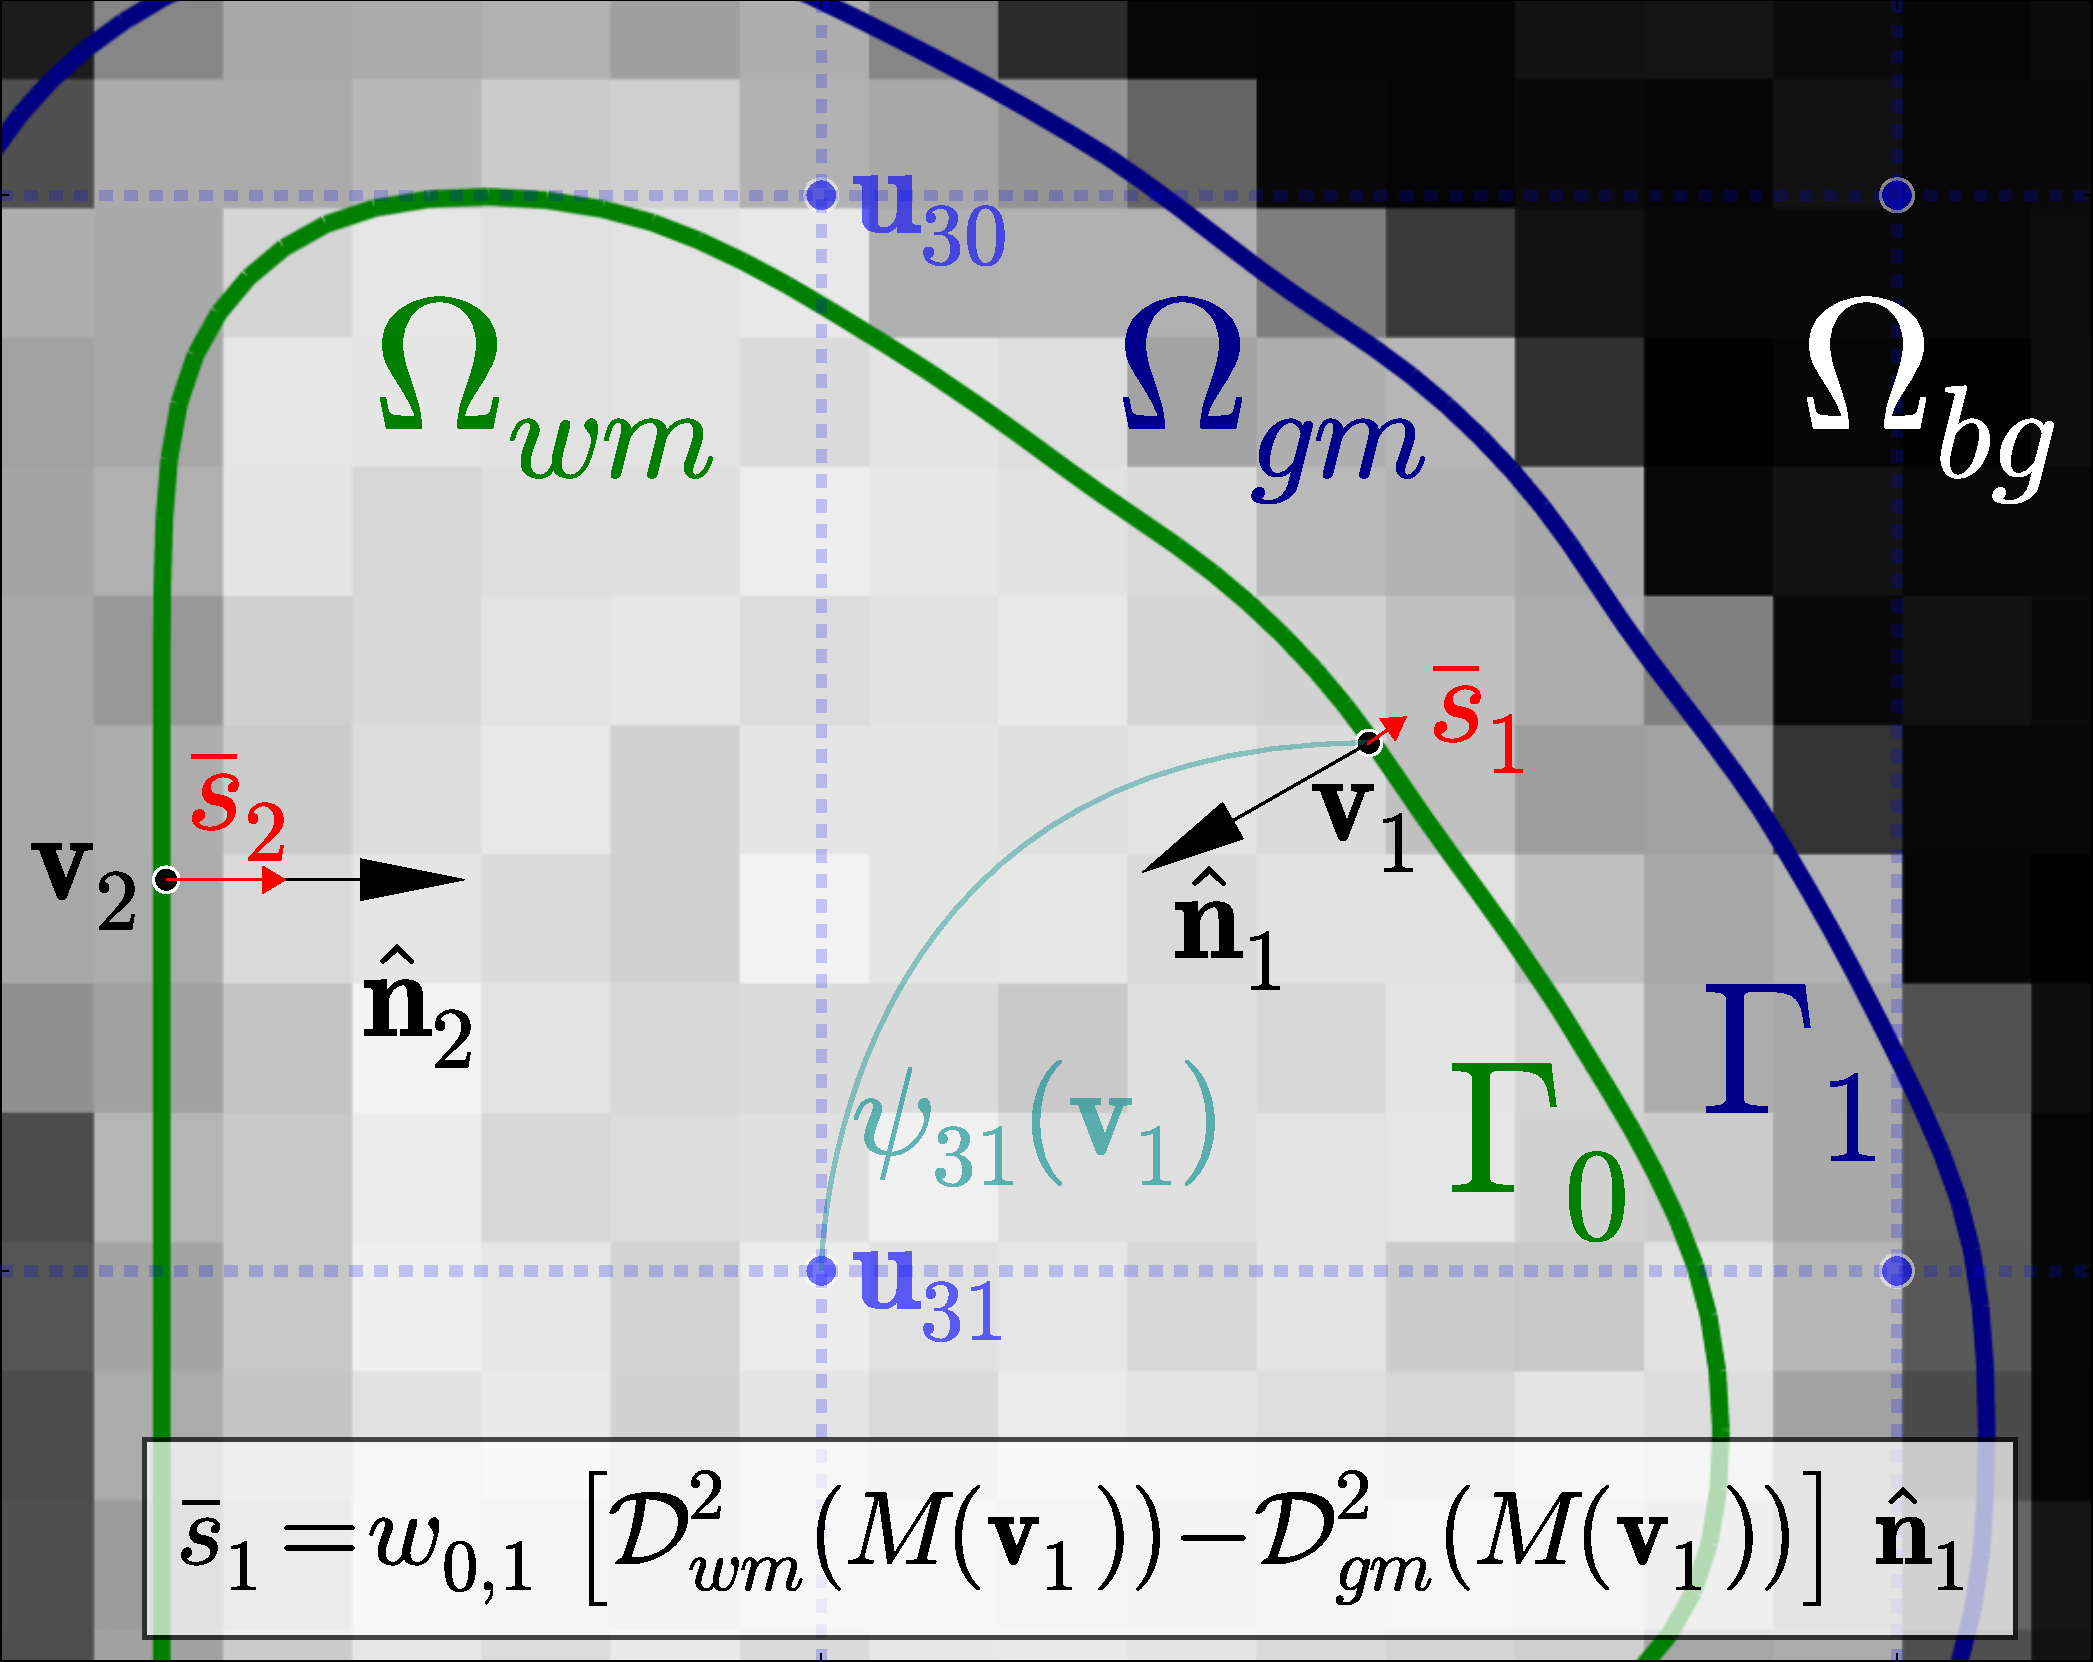
\includegraphics[width=\linewidth]{figure01}
  \caption{The active contours are defined as the interfacing surfaces of the competing
    \glspl{roi} $\Omega_i$, which
  are represented in green and dark blue in this close-up.
  They evolve iteratively following their inward normals $\hat{n}_i$ at each vertex
    $\vec{v}_i$ of the mesh.
  The gradient speeds $\bar{s}_i$ drive registration, which are computed as the disparity of the data
    energies with respect to the two limiting regions of $M(\vec{v}_i)$, the features of the image
    $M$ in the location of vertex $\vec{v}_i$ (see \suppl{equation SM5}).
  In this figure, $\bar{s}_1$ is written in the lower
    box, with $\Omega_{wm}$ in the inner limiting region, $\Omega_{gm}$ the outer region, and
    $w_{0,1}$ is the relative area associated with vertex $\vec{v}_1$ with respect to
    the total area of surface $\Gamma_0$.
      }\label{fig:regseg-method}
\end{figure}

\paragraph*{Deformation model}\label{sec:regseg-deformation_model}
Since the vertices of the surfaces $\{\vec{v}_i: \vec{v}_i \subset \gammaset \}_{i=1 \ldots N_V}$
  are probably located off-grid, it is necessary to derive $\vec{u}_i = \vec{u}(\vec{v}_i)$ from a discrete set of parameters
  $\{\vec{u}_k\}_{k=1 \ldots K}$.
Densification is achieved using a set of associated basis functions $\psi_k$ \eqref{eq:regseg-nodes_tfm}.
In our implementation, $\psi_k$ is selected as a tensor-product B-spline kernel
  of degree three.

  \begin{equation}
  \vec{v}_i' = \vec{v}_i + \vec{u}_i = \vec{v}_i + \sum_k \psi_k(\vec{r}) \: \vec{u}_k.
  \label{eq:regseg-nodes_tfm}
  \end{equation}


\paragraph*{Optimization}
\label{sec:regseg-gradient_descent}
To find the minimum of the energy functional \eqref{eq:regseg-energy},
  we propose a gradient-descent approach with respect to the underlying
  deformation field using the following \gls*{pde}:

  \begin{equation}
  \frac{\partial \vec{u}(\vec{r},t)}{\partial t} \propto - \frac{\partial E(\vec{u})}{\partial \vec{u}_k},
  \label{eq:regseg-general_gradient_descent}
  \end{equation}
  where $t$ is an artificial time parameter of the contour
  evolution and $\vec{u}_k$ are the parameters that support the estimate
  $\hat{U}$ of the transformation at the current time point.
Let us assume that the anisotropy is aligned with the imaging axes to simplify
  \eqref{eq:regseg-energy} as expression \eqref{eq:regseg-app_energy} in \ref{app:reg_term},
  and thus to compute its derivative \eqref{eq:regseg-general_gradient_descent}:

  \begin{align}
  \frac{\partial E(\vec{u})}{\partial \vec{u}_k} &=
  \frac{ \partial }{\partial \vec{u}_k} \Big\{
  \underset{l}{\sum} \int_{\Omega_l} \mdist{f'}{l} \,d\vec{r} \, +   \int_{\Omega} \frac12 [ \boldsymbol{\alpha} \cdot \vec{u}^{\circ2}
  + \boldsymbol{\beta} \cdot (\nabla \vec{u})^{\circ2} ] \,d\vec{r}
  \Big\},
  \label{eq:regseg-gradient_descent}
  \end{align}
  where $\vec{u}^{\circ2} = \vec{u}^T \cdot \vec{u}$.
Then, the data and regularization terms are split and discretized to compute their
  derivatives.
The computation of the explicit shape gradients at each $\vec{v}_i'$ is illustrated in \autoref{fig:regseg-method}.
Then, \eqref{eq:regseg-gradient_descent} can be reformulated as (see \suppl{equations SM6-SM12}):

  \begin{align}
  \frac{\partial E(\vec{u})}{\partial \vec{u}_k} &=
  \vec{g}_k  + \boldsymbol{\alpha} \cdot \vec{u}_k - \boldsymbol{\beta} \cdot (\Delta \vec{u}_k).
  \label{eq:regseg-final_gradient}
  \end{align}

Finally, to descend this gradient, we establish a semi-implicit Euler scheme (see \suppl{section S1.3}),
  with a step size parameter $\delta$, which we solve in the spectral domain as follows:

  \begin{align}
  \vec{u}_k^{t+1} = \mathcal{F}^{-1}\left\{ \frac{\mathcal{F}\{\delta^{-1} \, \vec{u}_k^t - \vec{g}_k\} }                  {\mathcal{F}\{(\delta^{-1} + \boldsymbol{\alpha})\, I - \boldsymbol{\beta}\Delta\}} \right\},
  \label{eq:regseg-update_equation}
  \end{align}
  where $I$ denotes the identity operator.


\paragraph*{Implementation details, settings, and convergence}
\label{sec:regseg-conv_report}
The \regseg{} tool includes a multiresolution strategy on the free-form deformation field.
Registration pyramids are created by setting the spacing between the control points of the B-spline basis
  functions for each level of the multiresolution strategy.
The implementation details as well as other features (such as the sparse matrix approach
  to fast interpolation) and the main parameters
  (such as $\delta$, $\boldsymbol{\alpha}$, $\boldsymbol{\beta}$, the B-spline grid resolutions,
 and target image smoothing) are discussed in \suppl{section S1}.
The actual choices of the parameter settings are publicly distributed with the source code for the experiments.
The final settings were obtained manually based on feedback from the post-registration convergence
  reports (such as that found in \suppl{section S1.3}).
We released \regseg{} along with the tool to generate the convergence report.

\subsection{Evaluation protocol}\label{sec:regseg-evaluation_protocol}
In order to assess the performance of \regseg{}, we defined the following general
  evaluation protocol:
1) Extract the set of undistorted surfaces $\gammaset_R$;
2) Compute a ground-truth field of displacements $U_\text{true}$, which is applied to
  generate warped images ($M$) for segmentation;
3) Execute \regseg{} with $\gammaset_R$ and use the warped data as inputs; and
4) Perform a visual assessment and compute the error metrics.

The adaptation of this protocol to the simulated phantoms and real data is explained in the
  following sections.
A first proof of concept to demonstrate \regseg{} in phantoms with simple
  geometries is introduced, using $U_\text{true}$ without directional restrictions.
Then, a more realistic environment with $U_\text{true}$ restricted to the
  \gls*{pe} axis of real \gls*{dmri} datasets is presented.

\subsection{Simulated phantoms}\label{sec:regseg-digital_phantoms}
The workflow required to simulate the digital phantoms and to assess the performance of
  \regseg{} with them is presented in \autoref{fig:regseg-evphantoms}.
A set of four binary objects (i.e., ``box'', ``ball'', ``L'',
  and ``gyrus'') was generated by combining the binarization of
  analytical shapes and mathematical morphology.
The reference surfaces $\gammaset_R$ were extracted from the binary shapes
  using \emph{FreeSurfer} tools \citep{fischl_freesurfer_2012}.
The ground-truth distortion was generated using a chain of two displacement
  fields supported by grids of B-spline basis functions.
The coefficients of the basis functions were generated randomly for
  both levels in their three dimensions.
The three components of the displacements $\vec{u} = (u_d)$
  were bounded above by 40\% of the separation between the control points
  at each level to obtain diffeomorphic transforms
  after concatenation \citep{rueckert_diffeomorphic_2006}.
The first deformation field was applied to generate large warpings
  with control points separated by 50.50 mm in the three dimensions
  ($u_d\leq$ 20.20 mm).
With the second warping, we aimed to obtain a field with smoothness
  close to that found in a typical distortion field of \gls*{dmri} data
  \citep{irfanoglu_susceptibility_2011}.
Therefore, the control points were separated by 25.25 mm ($u_d\leq$ 10.10 mm).
After generating the ground-truth deformation, the original surfaces
  were warped by interpolating the displacements field at each vertex.
The warped surfaces $\gammaset_\text{true}$ were binarized to generate tissue fractions
  at low (\isores[mm]{2.0}) and high (\isores[mm]{1.0}) resolutions.
Using a \gls*{mr} simulator \citep{caruyer_phantomas_2014}, we synthesized
  \gls*{t1} (TE/TR= 10/1500 ms) and \gls*{t2} images (TE/TR= 90/5000 ms), which
  corresponded to each phantom type, with each at two resolutions
  (1.0 mm and 2.0 mm isotropic).
The field of view at both resolutions was \isores[mm]{100}.
Next, \regseg{} was applied to map $\gammaset_R$ onto the warped phantoms to
  obtain the registered surfaces ($\hat{\gammaset}_\text{test}$).
To quantify the misregistration error, we computed the Hausdorff distance between
 $\hat{\gammaset}_\text{test}$ and $\gammaset_\text{true}$ using \citep{commandeur_vtk_2011}.

\begin{figure*}
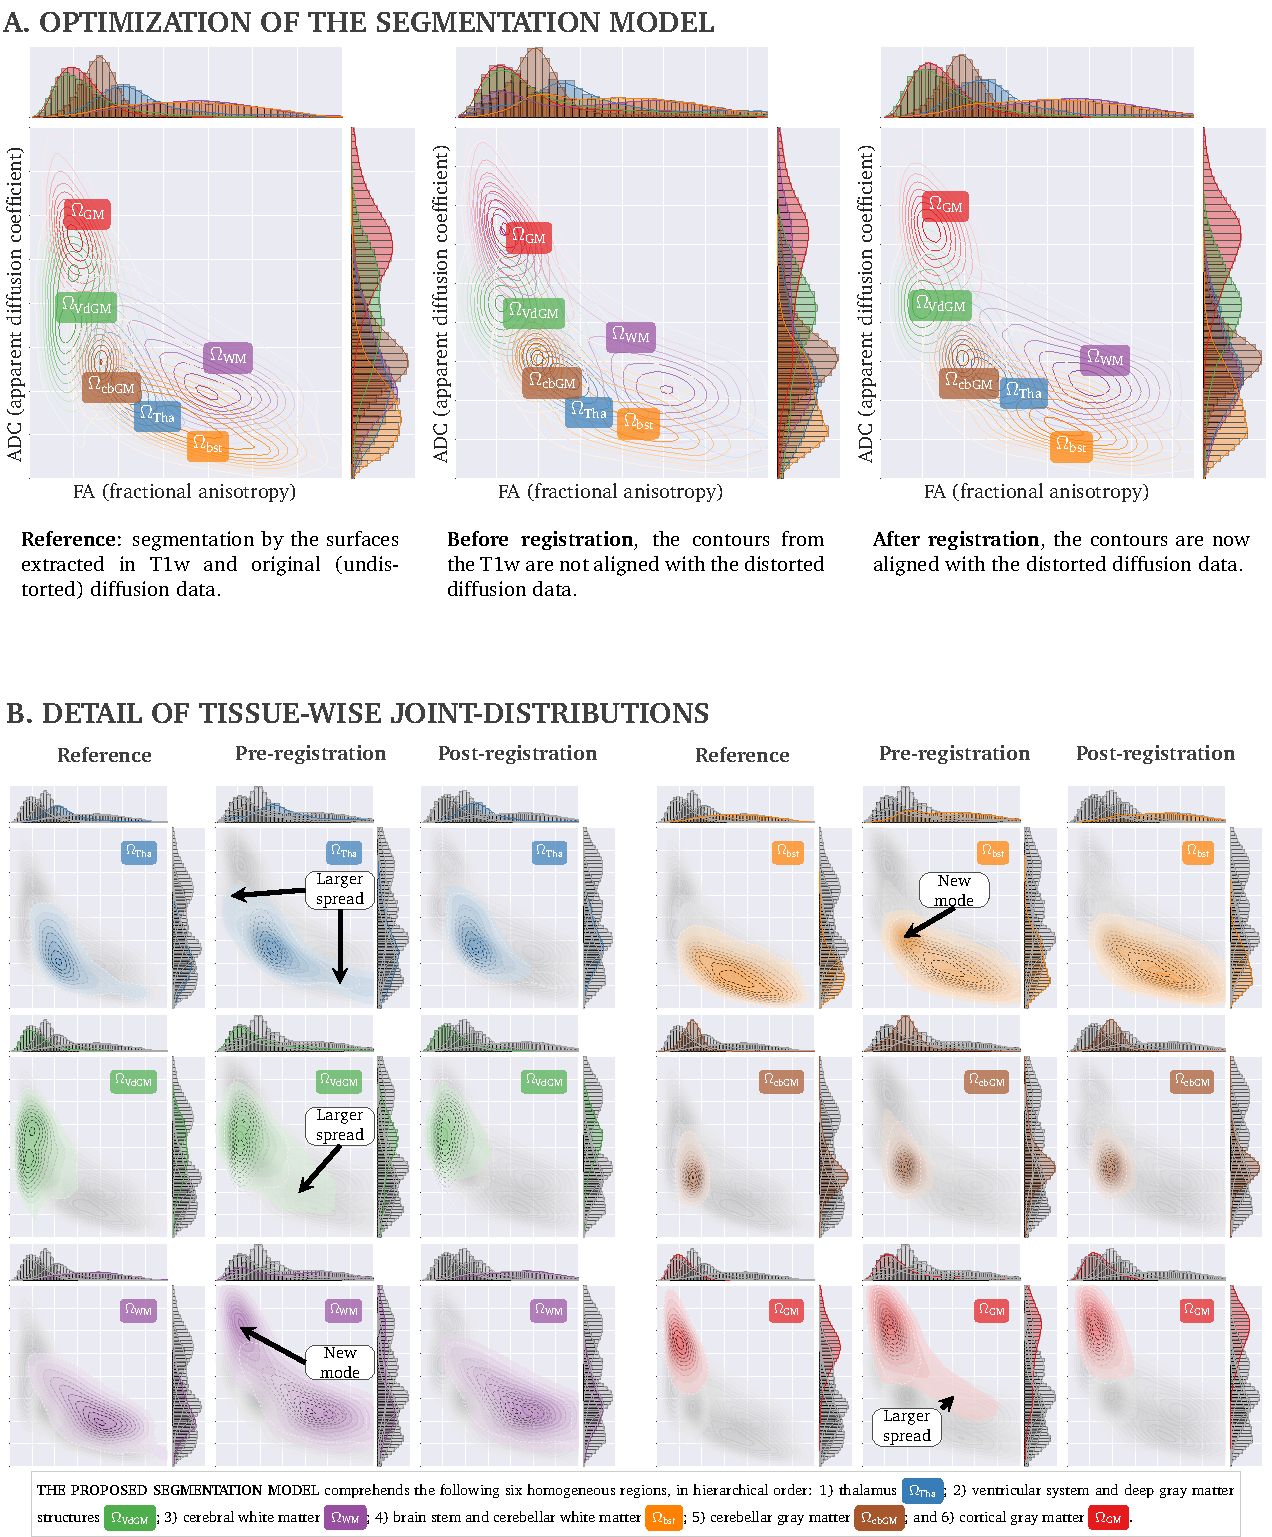
\includegraphics[width=\linewidth]{figure02}
\caption{Evaluation of \regseg{} using phantom data according to the following instrumental workflow.
  1) The reference surfaces $\gammaset_R$ are triangularized meshes extracted from the four binary shapes (i.e., ``box'', ``ball'', ``L'', ``gyrus'').
  2) A ground-truth displacement field was generated as described in \autoref{sec:regseg-digital_phantoms}, and applied to warp
      $\gammaset_R$, thereby obtaining $\gammaset_\text{true}$.
  3) After being warped, $\gammaset_\text{true}$ were projected onto the corresponding discrete 3D volume and downsampled to create partial volume effects at two resolutions,
     i.e., \isores[mm]{2.0} and \isores[mm]{1.0}, thereby producing sets of tissue fractions maps.
  4) The tissue fractions were fed into a \acrfull*{mr} simulator, which generated \acrfull*{t1} and \acrfull*{t2} -like images at the
     two possible resolutions.
  5) The \regseg{} tool was applied using the warped test images as multispectral moving images and $\gammaset_R$ as shape priors.
  6) The agreement between the surfaces fitted by \regseg{} ($\hat{\gammaset}_\text{test}$) and $\gammaset_\text{true}$ were assessed
     visually using automatically generated visual reports and quantitativelly with the Hausdorff distance between the
     corresponding surfaces.}\label{fig:regseg-evphantoms}
\end{figure*}


\subsection{Real datasets} \label{sec:regseg-human_connectome}
The general experimental framework for the real datasets is presented in \autoref{fig:regseg-evworkflows},
which extends our previous evaluation \citep{esteban_simulationbased_2014} of distortions
  using \gls*{dmri} phantoms.

\begin{figure*}
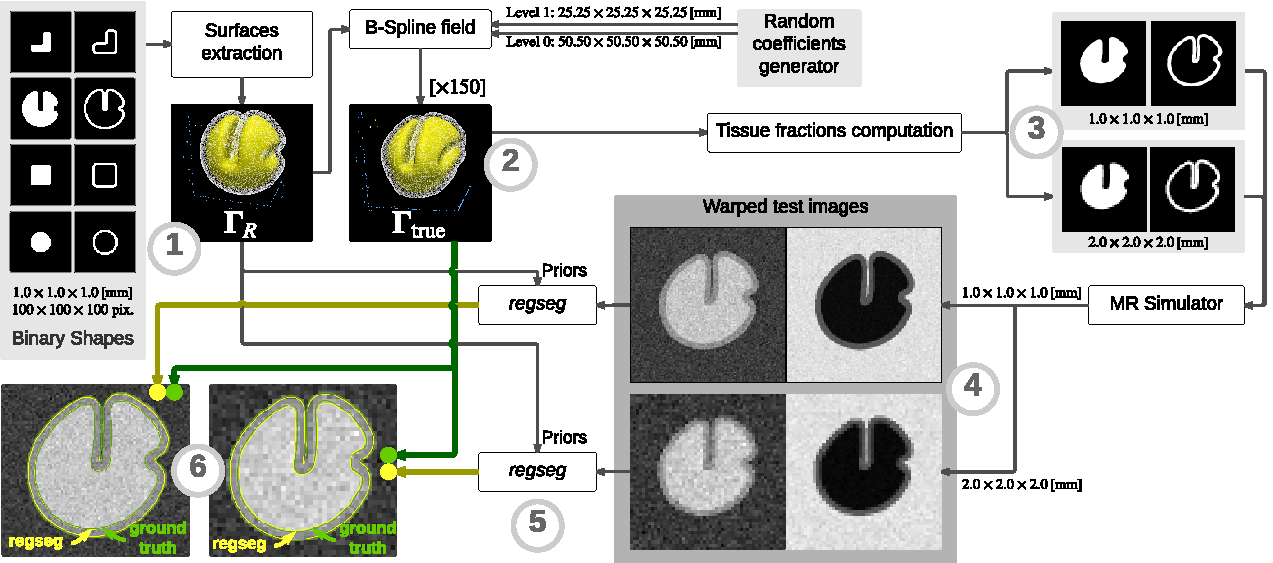
\includegraphics[width=\linewidth]{figure03}
\caption{Experimental workflow employed to process real data from the \acrfull*{hcp}.
  1) $\gammaset_R$ were extracted from the anatomical reference (\gls*{t1} image).
  2) For use as the ground truth, we generated a plausible synthetic distortion $U_\text{true}$
    from the field map with \eqref{eq:regseg-fieldmap}.
  3) The \gls*{dmri} data were warped using $U_\text{true}$ to reproduce the effects of real
    susceptibility-derived distortions.
  Target diffusion scalars (\gls*{fa} and \gls*{adc}) were computed with the distorted data and
    stacked to feed the multivariate input required by \regseg{}.
  4) The method was run to obtain $U_{test} = \hat{U}_{true}$, i.e., the estimate of
    the ground-truth deformation.
  5) The results were evaluated visually and quantitatively.}\label{fig:regseg-evworkflows}
\end{figure*}


\paragraph*{Data}
To evaluate \regseg{} using real \gls*{dmri} data obtained from human brains,
  we collected 16 subjects from the \gls*{hcp} database.
The original acquisitions are released within ``unprocessed'' packages, whereas
  the ``minimally preprocessed'' packages contain the corresponding images after
  some processing (correction for several artifacts, brain-extraction, spatial
  normalization, etc.).
We refer the reader to \citep{essen_human_2012} for exact details of the acquisition
  parameters and \citep{glasser_minimal_2013} for the preprocessing issues.
These datasets comprise a large set of images, including \gls*{t1}, \gls*{t2}, and
  multi-shell \gls*{dmri} images.

\paragraph*{Segmentation model}
Based on our experience   and previous studies \citep{ennis_orthogonal_2006},
  we defined the moving image as a stack of the \gls*{fa} and \gls*{adc} maps derived
  from \gls*{dmri} data.
After evaluating several alternative models, we empirically defined a partition \omegaset{}
  according to the following six regions:
  1) thalamus ($\Omega_{Tha}$);
  2) ventricular system and deep \gls*{gm} structures ($\Omega_{VdGM}$);
  3) cerebral \gls*{wm} ($\Omega_{WM}$);
  4) brain stem and cerebellar \gls*{wm} ($\Omega_{bst}$);
  5) cerebellar \gls*{gm} ($\Omega_{cbGM}$); and
  6) cortical \gls*{gm} ($\Omega_{GM}$).
Using tools in \emph{FreeSurfer} and appropriate selections of labels in the
  \emph{aparc} segmentation released with the \gls*{hcp} data, we extracted the $\gammaset_R$ set for the
  reference surfaces.
The segmentation model corresponding to this partition is shown in \autoref{fig:regseg-model}
  and discussed in greater detail in \suppl{section S4}.

\paragraph*{Ground-truth generation}
Realistic deformation is achieved by generating displacements fields that satisfy the theoretical
  properties of distortion \citep{jezzard_correction_1995}.
The displacements along the \gls*{pe} axis of the \gls*{dmri} image are related to the local
  deviation of the field $\Delta B_0(\vec{r})$ from its nominal value $B_0$, as follows:

  \begin{equation}
  u_\text{PE} = \frac{\gamma \, T_{acq}\, s_\text{PE}}{2\pi}\Delta B_0(\vec{r})\text{ [mm]},
  \label{eq:regseg-fieldmap}
  \end{equation}
where $\gamma$ is the gyromagnetic ratio, $T_{acq}$ is the readout time, and
  $s_\text{PE}$ is the pixel size along \gls*{pe}.
Certain \gls*{mr} sequences are designed to estimate $\Delta B_0$, thereby obtaining
  the so-called field map.
We derived the deformation $U_\text{true}$ from the field map image released with
  the corresponding packages of each dataset in the \gls*{hcp}.
The field map was unwrapped\footnote{fieldmaps are phase maps, which are intrinsically clipped in the interval
  of $[-\pi, \pi)$ [rads] or [rads/s].} and smoothed before applying \eqref{eq:regseg-fieldmap}.
Next, the original \gls*{dmri} was warped using the resulting displacement field and fed into
  a pipeline to process the corresponding \gls*{dti}, thereby computing the derived scalars of
  interest (\gls*{fa} and \gls*{adc}) using \emph{MRtrix} \citep{tournier_mrtrix_2012}.

\paragraph*{Metric assessment}
Initially, we investigated the appropriateness of the segmentation model.
For five test datasets, we uniformly sampled the space of distortions
  $\hat{U} = \epsilon \cdot U_\text{true} = \vec{r} + \epsilon \, u_\text{PE}$
  (with $\epsilon \in [-1.1, 1.1]$ and $u_\text{PE}$ from \eqref{eq:regseg-fieldmap}),
  and we evaluated the data term of the cost function \eqref{eq:regseg-energy}.
The minimum of the cost function (\autoref{sec:regseg-methods_map}) was consistently located at
  $\epsilon=0.0$ (the ground-truth) for all of the cases (\suppl{Figure S2}).

\paragraph*{Cross-comparison}
A similar workflow to the general evaluation framework used for \autoref{fig:regseg-evworkflows}
  was employed to integrate the alternate \gls*{t2b} registration scheme.
We reproduced the solution and settings provided with \emph{ExploreDTI}
  \citep{leemans_exploredti_2009}, which is a widely used toolkit for tractography analysis of
  \gls*{dti}.
\emph{ExploreDTI} internally employs \emph{elastix} \citep{klein_elastix_2010} to
  perform registration.

\paragraph*{Error measurement}\label{sec:regseg-experiments_evaluation}
Distortion only occurs along the \gls*{pe} axis of the image, so we computed the
  \gls*{swindex} as the area-weighted distance between the corresponding vertices of
  $\gammaset_{true}$ and their estimate obtained by the method under the test $\hat{\gammaset}_\text{test}$:

  \begin{equation}
  sWI = \frac{1}{\sum_i a_i} \sum\limits_i^{N_V} a_i\,\|
  \vec{v}_i - \hat{\vec{v}}_i \|,
  \label{eq:regseg-swindex}
  \end{equation}
  where $\vec{v}_i \subset \gammaset_\text{true}$ are the locations of the total $N_V$ vertices
  and $\hat{\vec{v}}_i \subset \hat{\gammaset}_\text{test}$ are the recovered locations
  that correspond to $\vec{v}_i$.
In practice, we only report the \gls*{swindex} for three surfaces of crucial interest in whole-brain
  tractography.
These three surfaces delineated the following regions in the model: $\Omega_{VdGM}$, $\Omega_{WM}$, and $\Omega_{GM}$. 
\makeatletter{}\section{Results}
\label{sec:regseg-results}

\subsection{Proof of concept using digital phantoms}
\label{sec:regseg-results_phantom}

\begin{figure*}
  \centering
  \includestandalone[width=\linewidth]{figure05}
  \caption{A. Visual assessment of the results obtained with the low resolution sets:
    ``gyrus'' (top left), ``L'' (top right), ``ball'' (bottom left),
    and ``box'' at (bottom right).
  The contours recovered after registration are represented in yellow.
  \Regseg{} achieved high accuracy because it determined the almost exact locations of the registered
    contours with respect to their ground truth positions (shown in green).
  The partial volume effect makes segmentation of the sulci a challenging problem with voxel-wise
    clustering methods, but they were successfully segmented with \regseg{}.
  B. Quantitative evaluation of registration errors in terms of the average Hausdorff distances between
    surfaces at low (left) and high (right) resolutions, which demonstrate that the errors were
    consistently below the size of the voxels.
    }\label{fig:regseg-phantom}
\end{figure*}
In total, 1200 experiments (four phantom types $\times$ 150 random warpings $\times$ two resolutions) were
  performed according to the workflow illustrated in \autoref{fig:regseg-evphantoms}.
For each experiment, the misregistration error was measured using the Hausdorff distance
  (see \autoref{sec:regseg-experiments_evaluation}) between the theoretical $\gammaset_\text{true}$ and
  the estimate obtained by \regseg{} ($\hat{\gammaset}_{test}$).
The results demonstrated that the accuracy was consistent and high, and below the image resolution.
\autoref{fig:regseg-phantom} (block C) shows the violin plots for each model type corresponding
  to the two sets of resolutions for the generated phantoms.
In order to relate the average misregistration error to the resolution of the moving image,
  we proceeded as follows.
First, we confirmed that the vertex-wise error distributions were skewed by using Shapiro-Wilk's test of
  normality.
All of the distributions of errors in the tests (four phantom types $\times$ two resolutions) were
  non-normal with $p<0.001$.
Consequently, we used the non-parametric Wilcoxon signed-rank test with the Bonferroni
  correction for multiple comparisons ($N=150$, for each phantom type).
The average errors were significantly lower than the voxel size with $p < (0.001 / 150)$
  in all tests (four phantom types $\times$ two resolutions).
Statistical tests might not be sufficiently conclusive, so we also computed the confidence intervals,
  as shown in \autoref{tab:ci_phantom}.


\begin{table}
    \centering
    \footnotesize
    \tabcolsep=0.1cm
    \begin{tabular}{lccccc}
    Res.   & ``gyrus'' & ``ball''  & ``box''   & ``L''     & Aggreg.    \\\hline
    1.0mm  & 0.18-0.38 & 0.31-0.45 & 0.34-0.42 & 0.34-0.40 & 0.34-0.38  \\
    2.0mm  & 0.59-0.60 & 0.65-0.76 & 0.68-0.71 & 0.67-0.77 & 0.64-0.66  \\
    \hline
    \end{tabular}
    \caption{The distributions of vertex-wise Hausdorff distances between the ground-truth surfaces and their
    corresponding estimates obtained with \regseg{} presented a 95\% CI below the half-voxel size for all of 
    the phantom types.
    The CIs were computed by bootstrapping using 10$^4$ samples, with the median as the location statistic.}\label{tab:ci_phantom}
\end{table}

\subsection{Evaluation using real datasets and cross-comparison}\label{sec:regseg-results_hcp}
Finally, we compared the performance of \regseg{} with that of the standard \gls*{t2b}
  method.
Summary reports for visual assessment of the 16 cases are included in \suppl{section S5}.
In \autoref{fig:regseg-results_real}, box A, the visual report is shown for one subject.
We computed the \gls*{swindex} \eqref{eq:regseg-swindex} of every surface after registration
  using both the \regseg{} and \gls*{t2b} methods.
Finally, to compare the results, we performed Kruskal-Wallis H-tests
  (a non-parametric alternative to ANOVA) on the warping indices for the three surfaces of 
  interest selected in \autoref{sec:regseg-experiments_evaluation}
  ($\Gamma_{VdGM}$, $\Gamma_{WM}$, $\Gamma_{pial}$).
All of the statistical tests showed that the error distributions obtained with \regseg{} and
  \gls*{t2b} were significantly different, and the violin plots in box B of
  \autoref{fig:regseg-results_real} demonstrate that the errors were always larger with \gls*{t2b}.
We also show the 95\% CIs of the \gls*{swindex} for these surfaces.
The aggregate CI for \regseg{} was 0.56--0.66 [mm], whereas the \gls*{t2b} method
  yielded an aggregate CI of 2.05--2.39 [mm].
The results of the statistical tests and the CIs are summarized in \autoref{tab:results_real}.



\begin{table}
    \centering
    \footnotesize
    \tabcolsep=0.08cm
    \begin{tabular}{cccccc}
    & & $\Gamma_{VdGM}$  & $\Gamma_{WM}$ & $\Gamma_{pial}$ & Aggreg. \\
    \hline
    \multirow{2}{*}{CI}
       & \regseg{}        & 0.50 - 0.78 & 0.50 - 0.55 & 0.66 - 0.73 & 0.56 - 0.66 \\
       & T2B                  & 1.78 - 2.58 & 1.94 - 2.36 & 2.16 - 2.58 & 2.05 - 2.39 \\
    \hline
    \multirow{2}{*}{H-tests}
       & p-value  & 4.1$\times$10$^{-6}$& 2.3$\times$10$^{-6}$& 2.3$\times$10$^{-6}$ & 1.8$\times$10$^{-16}$ \\
       & H-stat   & 21.20               & 22.31               & 22.31                & 67.85              \\
    \hline
    \end{tabular}
    \caption{Statistical analysis of results obtained using real data, which show that \regseg{} performed better than
    the alternative \acrfull{t2b} method.
    The distribution of the errors computed for the surfaces of interest ($\Gamma_{VdGM}$, $\Gamma_{WM}$, $\Gamma_{pial}$)
      and the aggregate of all surfaces (Aggreg. column) had lower 95\% CIs with \regseg{}.
   The CIs in this table were computed by bootstrapping using the mean as the location statistic and with 10$^4$ samples.
    The Kruskal-Wallis H-tests indicated that there was a significant difference between the results obtained using \regseg{} and
      the \gls*{t2b} method.
    }\label{tab:results_real}
\end{table}

\begin{figure*}
  \centering
  \includestandalone[width=\linewidth]{figure06}
  \caption{A. Example of a visual assessment report, which was generated automatically by the evaluation tool.
    Each view shows one component of the input image (in this case, the \gls*{fa} map), the ground-truth locations
    of the surfaces (green contours), and the resulting surfaces obtained with the test method (yellow contours).
  The first two rows show axial slices for \regseg{} and the \acrfull*{t2b} method, while the last two rows
    show the corresponding sagittal views.
  The coronal view is omitted because it was the least informative due to the directional property
    of the distortions.
  Specific regions where \regseg{} outperformed \gls*{t2b} are enlarged.
  B. Violin plots of the error distributions for each surface, which show the voxel size of the \gls*{dmri} images
    (1.25 mm), thereby supporting the improved results obtained by \regseg{} with the proposed settings.
  }\label{fig:regseg-results_real}
\end{figure*}  
\makeatletter{}\section{Discussion}
\label{sec:regseg-discussion}

\paragraph*{Accuracy tests}
The hypothesis tested in our study was that reliable image registration can be performed
  by searching for homogeneous regions in a multispectral image, which correspond to precise contours
  from an atlas, or extracted from another image (i.e., a different time step).
We demonstrated that active contours without edges can be used successfully to drive a
  deformation supported by B-spline basis functions with digital phantoms.
We randomly deformed four different phantom models to mimic three homogeneous regions
  (\gls*{wm}, \gls*{gm}, and \acrlong*{csf}) and we used them to simulate \gls*{t1} and \gls*{t2}
  images at two resolution levels.
After registration with \regseg{}, we measured the Hausdorff distance between the
  projected contours obtained using the ground-truth warping and our estimates.
We concluded that the errors were significantly lower than the voxel resolution.
We also assessed the 95\% \gls*{ci}, which yielded an aggregate interval of
  0.64--0.66 [mm] for the low resolution phantoms (2.0 mm isotropic voxel) and
  0.34--0.38 [mm] for the high resolution phantoms (1.0 mm isotropic).
Therefore, we also concluded that the error was bounded above by half of the
  voxel spacing.

\paragraph*{Application to real data}
We designed \regseg{} as a method for segmenting \gls*{dmri} data by exploiting the
  anatomical information extracted from the corresponding \gls*{t1} image of the subject.
Applications in whole-brain tractography \citep{smith_tractbased_2006,craddock_imaging_2013}
  usually solve this problem with a two-step approach.
First, the images are corrected for nonlinear distortions using auxiliary acquisitions
  such as field maps \citep{jezzard_correction_1995}, \gls*{t2} images \citep{kybic_unwarping_2000}.
Second, the segmentation is projected from a reference \gls*{t1} image using linear
  registration \citep{greve_accurate_2009}.
\Regseg{} addresses this joint problem in a single step and it does not require any additional
  acquisition other than the minimal protocol using only \gls*{t1} and \gls*{dmri} images.
This situation is found commonly in historical datasets.

We evaluated \regseg{} in a real environment using the experimental framework presented
  in \autoref{fig:regseg-evworkflows}.
We processed 16 subjects from the \gls*{hcp} database using both \regseg{}
  and an in-house replication of the \acrfull*{t2b} method.
\Regseg{} obtained very high accuracy, with an aggregate 95\% \gls*{ci} of 0.56--0.66 [mm], which was
  below the pixel size of 1.25 mm.
The misregistration error that remained after \regseg{} was significantly lower ($p < 0.01$) than the
  error corresponding to the \gls*{t2b} correction according to Kruskal-Wallis H-tests
  (\autoref{tab:results_real}).
Visual inspections of all the results (\suppl{section S5}) and the violin plots in
  \autoref{fig:regseg-results_real} confirmed that \regseg{} performed better than the \gls*{t2b} method
  in our settings.
We carefully configured the \gls*{t2b} method using the same algorithm and the 
  same settings employed in a widely-used tool.
However, cross-comparison experiments are prone to so-called \emph{instrumentation bias}
  \citep{tustison_instrumentation_2013}.
Therefore, these results do not prove that \regseg{} \emph{is better than} \gls*{t2b}.
Our results suggest that \regseg{} is a reliable option in this application field.
In addition, the \gls*{t2b} may introduce an additional (and small) error during the necessary
  registration of \gls*{t2} in the \gls*{t1} space.

%   with the theory-based displacement field that can be estimated with fieldmaps. 


\makeatletter{}\section*{Conclusion}
\label{sec:regseg-conclusion}

\Regseg{} is a variational framework for the simultaneous segmentation and
  registration of 3D \gls*{dmri} data obtained from the human brain, where within-subject
  anatomical information is used as a reference.
The registration method segments the target multivariate image into several competing regions, which are
  defined explicitly by their limiting surfaces.
The surfaces are active and they evolve on a free-form deformation field supported by the B-spline basis.
A descent optimization strategy is guided by shape gradients computed on the current partition
  of the target image.
\Regseg{} uses active contours without edges and it searches for
  homogeneous regions within the image.
We tested \regseg{} using digital phantoms by simulating \gls*{t1} and \gls*{t2} \gls*{mri}
  warped with smooth random deformations.
The resulting misregistration of the contours was significantly lower than the image resolution
  of the phantoms.

We proposed \regseg{} for simultaneously segmenting and registering \gls*{dmri} data to
  their corresponding \gls*{t1} image from the same subject.
We demonstrated the accuracy of the proposed method based on visual assessments of the results
  obtained by \regseg{} and cross-comparisons with a widely used technique.
Moreover, \regseg{} does not require any images in addition to the minimal acquisition protocol,
  which only utilizes \gls*{t1} and \gls*{dmri}.
As well as the proposed application to \gls*{dmri} data, other potential uses of \regseg{} are
  atlas-based segmentation and tracking objects in time-series.


\section*{Availability and reproducibility statement}
\label{sec:regseg-availability}
We considered the reproducibility of our results as a design requirement.
Therefore, we used real data obtained from a publicly available repository
  (the Human Connectome Project \citep{essen_human_2012}) and all of the software
  utilized in this study is also publicly available.
\Regseg{} was implemented on top of ITK-4.6 (Insight Registration and 
  Segmentation Toolkit, \url{http://www.itk.org}).
The evaluation instruments (\autoref{fig:regseg-evworkflows}) were implemented using
  \emph{nipype} \citep{gorgolewski_nipype_2011} to assess their reproducibility.
All of the research elements (data, source code, figures, manuscript sources, etc.) involved in this study
  are publicly available under a unique package \citep{esteban_regseg_2015}.  

\makeatletter{}\section*{Author contributions}
All the authors contributed to this study.
OE implemented the method, designed and conducted the experiments, wrote the paper,
  simulated the phantoms, and prepared the real data.
DZ devised and drafted the registration method, generated early phantom datasets, and
  collaborated in the implementation of the method.
AD, MBC, and MJLC interpreted the results.
AD, MBC, MJLC, JPT, and AS advised on all aspects of the study.

\section*{Acknowledgments}
The authors thank Y. Alem\'an and G. Wollny for their thorough reviews of the manuscript,
  V. Estellers for early discussions at the beginning of this project,
  and L. A. Vese for her support during OE's research visits to her laboratory.
We also thank A. Leemans for kindly sharing a p-code version of \emph{ExploreDTI} from
  which the settings for \emph{elastix} could be extracted.

DZ was supported by the Swiss National Science Foundation under grants PBELP2-137727, 
  P300P2-147778, and NSF-DMS 1418812.
This study was supported by the Spanish Ministry of Science and Innovation
  (projects TEC-2013-48251-C2-2-R and INNPACTO XIORT), Comunidad de Madrid (TOPUS) and
  European Regional Development Funds, the Center for Biomedical Imaging
  (CIBM) of the Geneva and Lausanne Universities and the EPFL, as well as the
  Leenaards and Louis Jeantet Foundations. 


\appendix
\numberwithin{equation}{section}
\makeatletter{}\renewcommand{\theequation}{A.\arabic{equation}}
\renewcommand{\thesubsection}{Appendix \arabic{subsection}}

\section*{Appendix}

\subsection{Simplifying the regularization term}\label{app:reg_term}
The exponentials of the Thikonov regularization prior \eqref{eq:regseg-thikonov} have the general form
  $\vec{v}^T \mathbf{M} \vec{v}$.
If $\mathbf{M}$ is a $n \times n$ diagonal matrix such that $\mathbf{M} = \vec{m} \, \mathbf{I}_n$, 
  then:

\begin{equation*}
\vec{v}^T \mathbf{M} \vec{v} = \vec{m} \cdot (\vec{v}^T \mathbf{I}_n \vec{v}) = \vec{m} \cdot \vec{v}^{\circ2},
\end{equation*}
  where we have introduced the Hadamard power notation\footnote{The Hadamard power of a matrix or a vector
  is the power of its elements $\mathbf{M}^{\circ p} = ({m_{ij}}^{p})$}.

In general, the anisotropy is aligned with the imaging axes, so 
  $\mathbf{A}$ and $\mathbf{B}$ of \eqref{eq:regseg-energy} can be simplified to diagonal matrices, such that
  $\mathbf{A}= \, \boldsymbol{\alpha}\,\vec{I}_n$ and
  $\mathbf{B}= \, \boldsymbol{\beta}\,\vec{I}_n$.
By substituting into equation \eqref{eq:regseg-energy}, we obtain:

  \begin{align}
  E(\vec{u}) &= \const + \underset{l}{\sum} \int_{\Omega_l} \mdist{f'}{l} \,d\vec{r} +   \int_{\Omega} \frac12 \left[ \boldsymbol{\alpha} \cdot \vec{u}^{\circ2} + \boldsymbol{\beta} \cdot (\nabla \vec{u})^{\circ2} \right] \,d\vec{r}.
  \label{eq:regseg-app_energy}
  \end{align}  

\bibliographystyle{mystyle}
\bibliography{Remote}


\end{document}
